\scanpage{28}
\uline{Prop D} Soit $Y$ \deleted{\unsure{a}} une variété topologique purement de dim $i$, $N$ un espace topologique. Alors \deleted{\unsure{fixé|si}}, $\forall(y,n)\in Y\times N$, \deleted{\unsure{tt|et} $\nu(y,n)$ est \unsure{défini}} \deleted{$(y,n)$ est $\nu$-mobile ssi} Si $\nu\geq i$, $(y,n)$ \inserted{$\in Y\times N$} est $\nu$-mobile ssi $n\in N$ est $(\nu-i)$-mobile. Donc
\[
Y_{\nu}(Y\times N)=Y\times Y_{\nu-i}(N).
\]
\margin{\diagram{\begin{tikzcd}[row sep=1em]
N\text{ dévissable} \arrow[d,Leftrightarrow] & {} \\
Y\times N\text{ dévissable}\quad(Y\neq\varnothing) & {} \arrow[dl,Rightarrow] \\
\text{\uline{Prop B}} & {}\\
\text{(\unsure{sous|sans} réserve de Prop A)}
\end{tikzcd}}}
\figure{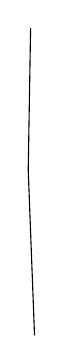
\begin{tikzpicture}\draw (0,0)--(-.08,2.1)--(-.05,3.9);\end{tikzpicture}}
\mspage{29}
